\section{Realization in fields and a harvesting model}
\label{sec:sharpness}

Two constructions show that the hypotheses and the rank
condition~\eqref{eq:rank} hold. Local perturbations of an arbitrary reference
field give four independent unfolding parameters, and a two-tier harvesting
model gives them through its natural parameters. In both cases we verify the
first-return geometry and use the standard unfolding to transfer the cycle
configurations.

\subsection{Local perturbations of a given reference field}
\label{subsec:specified-field}

Fix a nonstationary reference cycle \(\mathcal C\) satisfying the geometric
hypotheses of Section~\ref{sec:passage}, with passage strengths
\(A_{1,0}=-A_{2,0}\ne0\) and closing jets
\[
 R_0(0)=0,\qquad R_0'(0)=1,\qquad
 c_0=\tfrac12R_0''(0)\ne0.
\]
The positive penetration directions agree under the regular connections,
which have no additional seam crossing. Choose a second-contact box \(U_2\)
and a smooth closing-arc flow box \(U_3\), with disjoint closures away from
the first contact and return section.
Let \(\mathcal L_{\mathcal C}(U_2,U_3)\) be the finite-dimensional
jointly smooth parameter germs through this field with seam changes
supported in \(\operatorname{int}U_2\), inactive branch fixed there,
and active difference \(h_\lambda Z_\lambda\) with smooth
\(Z_\lambda\). In \(\operatorname{int}U_3\), which stays away
from the seam, a common smooth field may be added to both branches.
All other data are fixed. The perturbations that control \((m,\delta)\)
and \((a,b)\) have disjoint supports.

\begin{proposition}[Four independent unfolding parameters]
\label{prop:specified-rank}
Every such reference field admits a four-parameter unfolding in
\(\mathcal L_{\mathcal C}(U_2,U_3)\) with
\(D_\lambda(a,b,m,\delta)\) invertible at \(\lambda=0\), which reduces to the
reference field at \(\lambda=0\). The perturbations preserve matching,
regular seams, quadratic contacts and a one-turn first-return interval.
Every finite-parameter germ in \(\mathcal L_{\mathcal C}(U_2,U_3)\) is an
admissible family after a reduction depending on the germ.
\end{proposition}

\begin{proof}
Transport the first inactive integral along the unchanged first
connector. A Morse-type normalization of the clock near the second contact
gives
\[
 X_0^-=v(t,q)\partial_t,\qquad
 X_0^+=v(t,q)\{[1+(q-t^2)\alpha(t,q)]\partial_t
                    +(q-t^2)\mu(t,q)\partial_q\},\quad v>0.
\]
For a positive smooth \(e\),
\(h_0=e(q-t^2)\) and
\(eZ_0=v(\alpha\partial_t+\mu\partial_q)\).
Choose compactly supported cutoffs \(\psi_1,\psi_2\) in \(U_2\),
equal to one on a smaller contact core, and set
\begin{equation}\label{eq:specified-contact-controls}
 h_d=h_0-de\psi_1,\qquad
 X_{\kappa,d}^+=X_0^++(h_d-h_0)Z_0
                  +\kappa h_dv\psi_2e^{-1}\partial_q,
 \qquad X_{\kappa,d}^-=X_0^-.
\end{equation}
These changes extend by zero, recover \(X_0^\pm\) at zero, and satisfy
\[
 X_{\kappa,d}^+-X_0^-
 =h_d(Z_0+\kappa v\psi_2e^{-1}\partial_q).
\]
Thus the two fields agree on the moving seam.
In the core, \(z=q-d\) gives the normalized seam \(z=t^2\) and
coefficients \(v(t,z+d),\alpha(t,z+d),\mu(t,z+d)+\kappa\).
The contact is \((0,d)\), with inactive second seam derivative
\(-2v(0,d)^2<0\) in the normalized defining function, and the
active clock stays positive. Proposition~\ref{prop:quadratic-passage}
therefore gives \(A_2(\kappa,d)=\tfrac43[\mu(0,d)+\kappa]\).
The first passage and connector are unchanged, so
\begin{equation}\label{eq:specified-strength-jacobian}
 \delta=d,\quad m=A_{1,0}+\tfrac43[\mu(0,d)+\kappa],\qquad
 D_{(\kappa,d)}(m,\delta)(0)=
 \begin{pmatrix}4/3&(4/3)\mu_q(0,0)\\0&1\end{pmatrix}.
\end{equation}
The second strength is already transported; its incoming threshold is
\(\Gamma_1^{-1}(d)\).

In \(U_3\), use the base flow time \(s\) and the second out-port
coordinate transported by that flow as \(z\). Then
\(X_0^-=\partial_s\), the entrance holonomy is \(q\mapsto z=q\),
and the remaining transition is \(R_0\). Add to both branches
\[
 Y_\eta=\chi_1(s)\chi_2(z)(\eta_0+\eta_1z)\partial_z,
 \qquad \chi_1\ge0,\qquad \int\chi_1(s)\,ds=1,
\]
with compact support and \(\chi_2=1\) on a fixed transverse interval.
Small inputs and parameters stay in that interval, so the box
holonomy and closing transition are
\[
 H_\eta(z)=e^{\eta_1}z+\eta_0\phi(\eta_1),\qquad
 \phi(w)=\int_0^1e^{wt}\,dt,\qquad R_\eta=R_0\circ H_\eta.
\]
Consequently
\begin{equation}\label{eq:specified-four-jacobian}
 D_{(\eta_0,\eta_1,\kappa,d)}(a,b,m,\delta)(0)=
 \begin{pmatrix}
 1&0&0&0\\2c_0&1&0&0\\
 0&0&4/3&(4/3)\mu_q(0,0)\\0&0&0&1
 \end{pmatrix},\qquad \det=4/3.
\end{equation}
Disjoint supports make the closing leg independent of \((\kappa,d)\).
The inverse function theorem gives the local coordinates
\((a,b,m,\delta)\).

The seam $q-t^2-d\psi_1(t,q)=0$ has $q$ derivative greater than $1/2$
for small $d$ and agrees with the old seam on a boundary collar. The
reference has a positive angular clock on a fixed tube; matching gives
common local Lipschitz bounds for the perturbed fields.
Choose cores where the cutoffs are one, ports with strict transverse margins,
and strictly inactive connecting arcs, including the cutoff collars.
Proposition~\ref{prop:quadratic-passage} gives the first entry and the
first exit in each core, with second penetration $\Gamma_1(q)-d$.
Lemma~\ref{lem:common-tube} therefore gives the one-turn return
\[
 P_\lambda(q)=R_\eta\{d+
       \Gamma_{2,\kappa,d}(\Gamma_1(q)-d)\}.
\]
For any finite-parameter germ in \(\mathcal L_{\mathcal C}(U_2,U_3)\),
matching, smooth parameter dependence and the implicit function theorem at
the contact preserve these clock, core, port and positive transverse-derivative
margins after a reduction depending on the germ.
\end{proof}

\begin{corollary}[Cyclicity in the local perturbation class]
\label{cor:specified-cyclicity}
For every reference cycle \(\mathcal C\) of
Proposition~\ref{prop:specified-rank},
\(\operatorname{Cycl}(\mathcal L_{\mathcal C}(U_2,U_3),\mathcal C)=6\) in
the sense of Definition~\ref{def:cyclicity}. The corresponding suprema over
germs contained in \(\{m=0\}\), in \(\{\delta=0\}\) and in
\(\{m=\delta=0\}\) are four, four and two. The same values hold for the class
of all admissible families through the reference field.
\end{corollary}

\begin{proof}
Each germ is admissible after its own reduction, so
Proposition~\ref{prop:common-count} gives at most six fixed points in \(I\);
the same holds for every admissible family.
Remark~\ref{rem:cycle-fixed-point} identifies the isolated fixed points
in the common interval with the nearby limit cycles. Conversely,
Proposition~\ref{prop:specified-rank} and
Proposition~\ref{prop:single-scale-six} give six simple cycles
approaching \(\mathcal C\).
Restricting the same unfolding to the three slices,
Proposition~\ref{prop:sharp-slice-attainment} attains the bounds of
Corollary~\ref{cor:four-slices}. Since the families of
Proposition~\ref{prop:specified-rank} are admissible, the same values hold for
the class of all admissible families; this proves part~3 of
Theorem~\ref{thm:six-main}.
\end{proof}

\subsection{A two-tier escapement-harvesting model}
\label{sec:harvesting}

This model shows that the hypotheses and the rank condition hold for the
natural parameters of an ecological family. Continuous threshold harvesting,
which switches harvest on continuously above a population threshold, is
studied in~\cite{leardrebaza2011,rebaza2012}. The policy of Bohn, Rebaza and
Speer~\cite{bohn2011} stops prey harvest below a lower threshold, increases it
linearly between two thresholds and caps it above the upper one; Onana Ndzana
et al.~\cite{onana2019} use it in a delayed Leslie--Gower model with prey
refuge. We intensify harvest above the upper threshold, using the normalized
smooth
predator-harvesting core of Huang, Gong and Ruan
\cite[equation~(9) and Theorem~3.6]{huang2013}:
\begin{equation}\label{eq:harvesting:model}
 \dot x=x(1-x-y)-u(x-L)_+-v(x-U)_+,\qquad
 \dot y=y\left(d-\beta\frac yx\right)-h.
\end{equation}
Here \(x,y>0\) are prey and predator densities,
\(\beta,d,h,u,v>0\), and \(0<L<U<1\).
The predator parameters \(d,\beta,h\) describe growth, density limitation
relative to prey abundance, and constant-yield harvest.
The marginal prey efforts are \(0,u,u+v\). We work in a compact
subset of the positive quadrant. The middle smooth extension is
\begin{equation}\label{eq:harvesting:middle}
 F_c=x(1-x-y)-u(x-L),\qquad
 G=y(d-\beta y/x)-h,\qquad X_c=(F_c,G),
\end{equation}
and the exterior extensions are
\[
 X_\ell=(x(1-x-y),G),\qquad X_r=(F_c-v(x-U),G).
\]
The adjacent extensions agree on the whole seams:
\(X_\ell=X_c\) on \(x=L\) and \(X_c=X_r\) on \(x=U\).
The middle extension is
inactive at both contacts, with active sides outside \(L\le x\le U\).
The branches are analytic for \(x>0\) and the field is
locally Lipschitz.

\begin{theorem}[Natural harvesting realization]
\label{thm:harvesting-realization}
There exists \(\rho_0>0\) such that, for every fixed radius
\(0<\rho<\rho_0\) in the smooth-core fold construction of
Appendix~\ref{app:harvesting-fold}, there exists \(u_0(\rho)>0\) with the following
property. For every fixed \(0<u<u_0(\rho)\) there are positive parameters
\(\beta,d,h,v\) and thresholds \(0<L<U<1\), depending on \(\rho\) and \(u\),
for which \eqref{eq:harvesting:model} has an embedded semistable periodic
orbit \(\mathcal C\) with exactly two quadratic contacts, at its minimum and
maximum prey densities. In one transported return coordinate the contact
levels agree and
\[
 A_1=A_0=-A_2\ne0,\qquad
 R(0)=0,\qquad R'(0)=1,\qquad c_0=\tfrac12R''(0)<0.
\]
The map \(\lambda\mapsto(a,b,m,\delta)\) has rank four in the natural
family \(\lambda=(\beta,d,h,u,v,L,U)\). The cyclicity of \(\mathcal C\) in
this family is six, and the corresponding values on \(m=0\), on
\(\delta=0\) and on their intersection are four, four and two. The
conclusions of Theorems~\ref{thm:main-saturation-summary}
and~\ref{thm:actual-quartic-summary} hold for the standard unfolding of this
family (Corollary~\ref{cor:realization-transfer}).
\end{theorem}

We construct a smooth cyclic fold, fit the thresholds to its prey
extrema, and cancel the passage strengths with a positive effort
ratio. The directions \((\nu,L,v,U)\), with \(\beta,u\) fixed,
then give the standard unfolding.

\subsection{Threshold fitting, cancellation and closing curvature}

Appendix~\ref{app:harvesting-fold} constructs cyclic folds of
the smooth core, for every sufficiently small fixed radius \(\rho>0\).
The fold is embedded and nonstationary, lies in the positive quadrant,
and has exactly one nondegenerate prey minimum and maximum. In radial
coordinates its displacement satisfies
\eqref{eq:harvesting:fold-data}, with \(\ell<0\), and the
\((\beta,\nu)\) Jacobian of \((D,D_r)\) is invertible.
These strict properties allow the thresholds and positive efforts to be
fitted to a fixed fold.

For positive \(u\), use
\begin{equation}\label{eq:harvesting:perturbed-chart}
 y_e=\tfrac45-u(1-5L),\qquad
 d=8\beta+\tfrac15+\nu,\qquad h=y_e(d-5\beta y_e).
\end{equation}
The middle field vanishes at \((1/5,y_e)\). At \(u=0\) the chart
reduces to \eqref{eq:harvesting:core-chart} and is independent of
\(L\). Fix a positive fold radius in
\eqref{eq:harvesting:fold-data}. The invertible \((\beta,\nu)\)
Jacobian of \((D,D_r)\) continues a fold \(\mathcal C(u,L)\)
for small \(u,L-L_0\), where \(L_0\) is the unperturbed prey
minimum. Its curvature and two nondegenerate extrema persist.
For its minimum \(x_{\min}(u,L)\),
\(\partial_Lx_{\min}(0,L_0)=0\), so
\begin{equation}\label{eq:harvesting:threshold-fit}
 L=x_{\min}(u,L),\qquad U=\max_x\mathcal C(u,L(u))
\end{equation}
has a unique local smooth solution with \(0<L(u)<U(u)<1\).
After reducing \(u\), all parameters in
\eqref{eq:harvesting:perturbed-chart} remain positive. The fitted
orbit stays in the closed middle strip, touching its boundary only
at the extrema, and is an orbit of \eqref{eq:harvesting:model} for every \(v\). There
\(F_c=0\), \(F_{c,y}=-x\), and nonstationarity gives \(G\ne0\),
so
\begin{equation}\label{eq:harvesting:quadratic-contact}
 \ddot x=F_{c,y}G=-xG\ne0.
\end{equation}

Figure~\ref{fig:harvesting-orbit} illustrates this fitted threshold geometry.
For each of two fixed parameter tuples, Online Resource~3 proves by interval
arithmetic the existence of at least six distinct simple periodic orbits of
\eqref{eq:harvesting:model}. Theorem~\ref{thm:harvesting-realization} is analytic and does not depend on
these certificates.
\begin{figure}[tb]
 \centering
 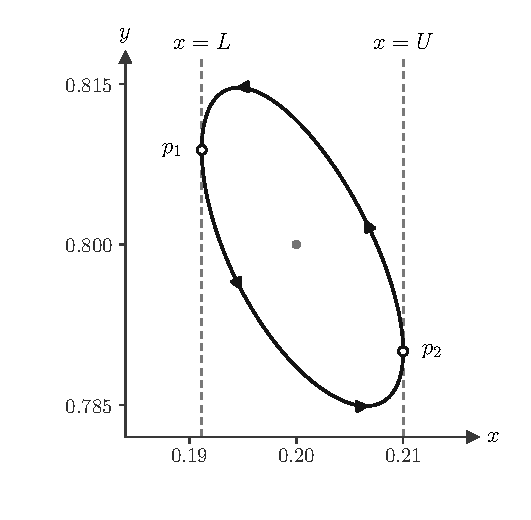
\includegraphics[width=90mm]{figures/harvesting-orbit.pdf}
 \caption{Numerical illustration of the fitted threshold geometry of
 \eqref{eq:harvesting:model}. With \(u=10^{-6}\) and \(U=0.21\)
 prescribed, the resulting parameter values are
 \(\beta\simeq0.031443254\), \(d\simeq0.451546877\),
 \(h\simeq0.260619080\), and \(L\simeq0.191154841\).
 The middle orbit touches the vertical thresholds \(x=L\) and \(x=U\)
 at its prey extrema. Open circles mark the contacts \(p_1,p_2\),
 arrows show increasing time, and the dot marks the middle
 equilibrium. Theorem~\ref{thm:harvesting-realization} proves the existence
 of such reference cycles and their six-cycle unfoldings.}
 \label{fig:harvesting-orbit}
\end{figure}

Positive penetration is outward, into \(x<L\) or \(x>U\).
At \(p_i=(x_i,y_i)\), write \(G_i=G(p_i)\).
Equation~\eqref{eq:harvesting:quadratic-contact} gives \(G_1<0<G_2\), so
\(y=y_i\) are transverse sections. In the coordinates \(z_1=L-x\),
\(z_2=x-U\), their inactive transitions along the forward arcs satisfy
\[
 S_1'(0)=-\frac{G_1}{G_2}
       \exp\!\int_{p_1}^{p_2}\operatorname{div}X_c\,dt>0,
 \qquad
 S_2'(0)=-\frac{G_2}{G_1}
       \exp\!\int_{p_2}^{p_1}\operatorname{div}X_c\,dt>0.
\]
Positive penetration normalizations preserve these signs and, on a common
smaller domain, give positive derivative margins.
Transport one inactive first integral \(I\) from the first box through
the connector to the second, with outward direction positive. These are
local first-integral charts joined along the connecting tube. At
\(p_i\), put \(\sigma_1=-1\), \(\sigma_2=1\),
\(s_i=I_x(p_i)\). Then \(I_y(p_i)=0\) and
\(\sgn s_i=\sigma_i\). A Morse-type normalization of the clock for
\(\mathfrak h_i=\sigma_i(x-x_i)\), preserving \(I\), gives
\begin{equation}\label{eq:harvesting:clock}
 \mathfrak h_i=e_i(t,I)(I-t^2),\qquad
 e_i(0,0)=\frac{\sigma_i}{s_i}>0,\qquad
 \dot t(0,0)=\omega_i
 =\sqrt{-s_iF_{c,y}(p_i)G(p_i)/2}>0.
\end{equation}
These clocks differ from the core frequency \(\omega\). For active
difference \(\mathfrak h_iZ_i\), the normalized transverse coefficient is
\[
 \mu_i(0,0)
 =\frac{e_i(0,0)}{\omega_i}dI(Z_i)
 =\frac{\sigma_i(Z_i)_x}{\omega_i}.
\]
Here \(Z_1=-u\partial_x\), \(Z_2=-v\partial_x\); thus
\eqref{eq:passage:strength-jet} gives
\begin{equation}\label{eq:harvesting:strengths}
 A_1=K_1u=\frac{4u}{3\omega_1}>0,\qquad
 A_2=-K_2v=-\frac{4v}{3\omega_2}<0.
\end{equation}
The opposing passage signs come from the opposite outward directions at
the two thresholds; both harvesting efforts are positive.
The inactive clocks and transport are independent of \(v\), so
the exact positive ratio
\begin{equation}\label{eq:harvesting:effort-relation}
 v=u\frac{K_1}{K_2}=u\frac{\omega_2}{\omega_1}
\end{equation}
cancels the strengths in the same transported coordinate.
Both contacts lie on one inactive orbit, so their levels agree.
Their passage derivatives equal one at the touch and the middle fold
has multiplier one. Lemma~\ref{lem:passage:finite-inverse} gives
\(Q(q)=q+q_+^{5/2}\mathcal L(\sqrt{q_+})\), with no terms of order
\(q^{3/2}\) or \(q^2\). The regular map \(R\) is the inactive monodromy.

The closing curvature \(c_0\) is negative in the outward-positive coordinate. First
set \(u=0\) and fix the cyclic-fold parameters at a small radius
\(\rho\). Vary the initial radial coordinate \(r\) with these
parameters fixed. Smooth finite-time normal-form flow has prey component
\[
 x(r,\theta)=\tfrac15+rp(\theta)+O(r^2+\rho^2r),
\]
where \(p\) is a nonzero first harmonic and the \(r\)-derivative
of the remainder is \(O(r+\rho^2)\). Its unique nearby prey minimum
\(M(r)\) satisfies \(M'(\rho)=-\gamma+O(\rho)<0\), \(\gamma>0\).
The minimum locus \(F_c=0\) is transverse, since its derivative
along the orbit is \(\ddot x\ne0\). If \(H(r)\) is the
transported inactive integral there, \(I_y=0\), \(I_x<0\) give
\(H'(\rho)=I_xM'(\rho)>0\). For the radial core return \(P_c\)
at these fixed parameters,
\(R=H\circ P_c\circ H^{-1}\). At the fixed point, where \(R'=1\),
\[
 R''(0)=\frac{P_c''(\rho)}{H'(\rho)}<0
\]
by \eqref{eq:harvesting:fold-data} and \(\ell<0\).
Continuation to fitted small positive \(u\) preserves this strict
sign and \(H'>0\). The cancelling composition has zero quadratic
defect, so \(c_0<0\) for the reference cycle as well.

\subsection{Rank condition and first return}

At the fitted orbit we now show that the four return-map controls can be
varied independently and that nearby orbits keep the first-return structure.

Use \((\nu,L,v,U)\) in \eqref{eq:harvesting:perturbed-chart}, with
\(\beta,u\) fixed. Choose the first incoming coordinate from the
middle extension and lower seam only. The regular monodromy \(R\)
is independent of \(v,U\): changes of the upper ports alter the
intermediate inactive holonomies but preserve their middle-return
composition. The threshold separation \(\delta\) is independent of
\(v\). At the upper tangency \(F_c(U,y_2(U))=0\) and \(I_y=0\),
so
\begin{equation}\label{eq:harvesting:upper-rank}
 \delta_U=I_x(p_2)\ne0,\qquad m_v=-K_2\ne0.
\end{equation}
Hence
\begin{equation}\label{eq:harvesting:rank-matrix}
 D_{(\nu,L,v,U)}(a,b,m,\delta)=
 \begin{pmatrix}
 a_\nu&a_L&0&0\\ b_\nu&b_L&0&0\\
 *&*&-K_2&*\\ *&*&0&\delta_U
 \end{pmatrix}.
\end{equation}
For the upper-left minor first set \(u=0\) at the fixed core fold.
The lower tangency is \(p_1(L)=(L,1-L)\); its level in an unchanged
core transverse coordinate has derivative
\begin{equation}\label{eq:harvesting:lower-level}
 \zeta_L=dI(p_1'(L))=I_x(p_1)\ne0.
\end{equation}
Choose this coordinate to agree with the incoming one at the base,
and centre the contact by \(T_L(\zeta(L))=0\). Then
\(R_L=T_L\circ P_c\circ T_L^{-1}\). Since at the fold
\(P_c(\zeta)=\zeta\) and \(P_c'(\zeta)=1\),
\begin{equation}\label{eq:harvesting:lower-rank}
 a_L=0,\qquad b_L=P_c''(\zeta)\zeta_L
                   =2c_0\zeta_L\ne0.
\end{equation}
At \(u=0\), the core return \(P_c\) is independent of \(L\), so the
\(L\)-dependence of \(R_L\) comes only from the moving section. Because
the base coordinates agree and \(D_r=0\), contact motion leaves the
offset derivative in \(\nu\) unchanged;
\eqref{eq:harvesting:scaled-return} gives \(a_\nu\ne0\). Moving-coordinate
terms in \(b_\nu\) do not enter the minor since \(a_L=0\). Thus the minor
is \(a_\nu\,2c_0\zeta_L\ne0\); another transverse scaling changes it
only by a nonzero factor. These objects extend smoothly to
\(u=0\), so at each fixed radius the minor persists for small
positive \(u\), with fitted thresholds and
\eqref{eq:harvesting:effort-relation}. All couplings remain in
\eqref{eq:harvesting:rank-matrix}, whose determinant is the minor
times \((-K_2)\delta_U\ne0\). The chart directions embed in
\((\beta,d,h,u,v,L,U)\), proving~\eqref{eq:rank} in the natural
parameters.

The fitted cycle is compact, embedded and nonstationary. On a fixed tube,
the vertical seams stay regular and the matched model has common local
Lipschitz bounds. The positive angular clock, transverse ports, positive
transverse-derivative margins and strictly inactive connectors persist under
small parameter changes. In each core,
\eqref{eq:harvesting:clock} and the smooth active difference satisfy the
passage hypotheses, including first entry and first exit.
Lemma~\ref{lem:common-tube} gives the chronological first return on one
common interval. Thus each constructed reference satisfies the geometric
first-return hypotheses as well as the rank condition.

\subsection{Transfer to the natural parameters}

\begin{corollary}[Main results in the constructed families]
\label{cor:realization-transfer}
For each reference constructed above, with its standard unfolding and
interval \(I\), the bounds and attainment of Theorem~\ref{thm:six-main} hold.
In the sign case $A_1(\lambda_0)=B>0$, $c_0=-C<0$, which includes every
harvesting reference, the conclusions of
Theorem~\ref{thm:main-saturation-summary}, Theorem~\ref{thm:actual-quartic}
and Proposition~\ref{quartic:strata} hold for the same unfolding on \(I\).
In the harvesting family all parameters remain positive and $0<L<U<1$.
\end{corollary}

\begin{proof}
The Jacobians \eqref{eq:specified-four-jacobian} and
\eqref{eq:harvesting:rank-matrix}, together with
Lemma~\ref{lem:common-tube}, give the standard unfolding and common interval.
Fix this unfolding before choosing the scale: every compact set of rescaled
controls lies in the domain of its inverse \(\Lambda\) at sufficiently small
scale. In the harvesting family the inverse maps \((a,b,m,\delta)\) to
\((\nu,L,v,U)\), with \(\beta,u\) fixed, preserving positivity and
$0<L<U<1$. Apply Theorems~\ref{thm:six-main}
and~\ref{thm:main-saturation-summary}. In the stated sign case,
Lemma~\ref{mainloc:all-roots} localizes all roots in \(I\): two simple
negative roots and a positive cluster beyond both thresholds.
Theorem~\ref{thm:actual-quartic} and Proposition~\ref{quartic:strata}
give its preparation and strata. Remark~\ref{rem:cycle-fixed-point}
identifies the isolated fixed points with cycles, completing
Theorem~\ref{thm:harvesting-realization}.
\end{proof}

\section{Concluding remarks}\label{sec:concluding}

A cancellation that makes the reference return map $C^2$ need not make its
unfoldings jointly $C^2$. The aligned cancelling slice has cyclicity two,
whereas a full-rank unfolding of all four return-map controls attains six
limit cycles. Several questions remain open.
\begin{enumerate}
\item Theorem~\ref{thm:main-saturation-summary} describes the limit of the
saturation domains. Apart from the fourfold point of
Theorem~\ref{thm:actual-quartic-summary} and the corner $S_4\to0$ treated in
Online Resource~1, the number of limit cycles at positive scale for parameters
near boundary points of $\mathcal K_4$ is not determined here.
\item Parts~2 and~3 of Theorem~\ref{thm:main-saturation-summary} and
Theorem~\ref{thm:actual-quartic-summary} are stated in the sign case
$A_1(\lambda_0)>0$, $c_0<0$. The remaining sign cases are not treated here.
\item A periodic orbit tangent to two switching lines of a discontinuous
system with sliding is studied in~\cite{roitenberg2025}. The effect of
cancelling leading terms in the presence of sliding is open.
\item The contacts here are quadratic. For tangencies of higher order the
corrections have other exponents, and the interaction between cancellation
and moving thresholds remains to be analysed.
\end{enumerate}
